% Document uses 12 pt font
% 1 in margins
% Contains a relative path for images

\documentclass [10pt]{article}

% page geometry 
\usepackage[margin=1in]{geometry}
\usepackage{changepage}

\usepackage{lscape}



% ----------  PACKAGES START ------------ %

% Table cell color package and highlighting
\usepackage[table]{xcolor}
\usepackage{color,soul}
\usepackage{colortbl}
\usepackage{float}
\usepackage{wrapfig}
\usepackage[rightcaption]{sidecap}
\usepackage{subfigure}
\usepackage{caption}
% VIC title package
\usepackage{cabin}
\usepackage[T1]{fontenc}

% default font package
%\usepackage{times}
\usepackage{helvet}
%\renewcommand{\familydefault}{\sfdefault}

% ---------- End Font Packages -------------- %

% Title Packages
\usepackage{titlesec}
\usepackage{titletoc}

% Image Package
\usepackage{graphicx}

% Table Packages
\usepackage{longtable}
\usepackage{multirow}
\usepackage{multicol}
\usepackage{multirow}
\usepackage{array}
\usepackage{tabularx}
\usepackage{colortbl}
\usepackage{listings}

\renewcommand{\arraystretch}{1.2}% Spread rows out evenly in table
\setlength{\LTpre}{0.5pt} % Reduces white space around tables (top)
%\setlength{\LTpost}{0pt} % Reduces white space around tables (bottom)
\setlength\arrayrulewidth{1pt}
%\setlength\minrowclearance{2pt}

%[.9\tabcolsep]

\definecolor{dkgreen}{rgb}{0,0.6,0}
\definecolor{gray}{rgb}{0.5,0.5,0.5}
\definecolor{mauve}{rgb}{0.58,0,0.82}
%Code listing style named "mystyle"
\lstdefinestyle{mystyle}{
  %backgroundcolor=\color{backcolour},  
  commentstyle=\color{codegreen},
  keywordstyle=\color{magenta},
  numberstyle=\tiny\color{codegray},
  stringstyle=\color{codepurple},
  basicstyle=\footnotesize,
  breakatwhitespace=false,         
  breaklines=true,                 
  captionpos=b,                    
  keepspaces=true,                 
  numbers=left,                    
  numbersep=5pt,                  
  showspaces=false,                
  showstringspaces=false,
  showtabs=false,                  
  tabsize=2
}
\lstset{style=mystyle}


% Color Packages
\usepackage{color}   
\definecolor{sectionC}{rgb}{0.95,0.52,.0}
\definecolor{subsectionC}{rgb}{1.0,.64,.26}
\definecolor{subsubsectionC}{rgb}{1.0,.87,.68}
\definecolor{tableCell}{rgb}{.98,.81,.69}


% List package
\usepackage{enumitem}
\setenumerate{itemsep=0pt, itemindent=0in,leftmargin=0.5in}


% Paragraph parameter

\setlength{\parindent}{0pt}


% ------------- Creates a linked Table of Contents  Start --------------- %
\usepackage{hyperref}
\hypersetup{
colorlinks=true, %set true if you want colored links
linktoc=all,     %set to all if you want both sections and subsections linked
linkcolor=black,}  %choose some color if you want links to stand out

% ------------- Creates a click-able Table of Contents  End--------------- %

% ---------- PACKAGES END ------------ %



% ------------------- START HEADER AND FOOTER ---------------------------%
\usepackage{fancyhdr}

% Helps with the n of total n pages
\usepackage{lastpage}

\pagestyle{fancy}

% Header
\lhead{Verification and Validation} 
\rhead{Revision: 0}
\fancyhead[LE, CO]{Group 9: LazyBots}

% Removes line under the header 
\renewcommand{\headrulewidth}{0pt}
\setlength{\headsep}{.2in}

% Footer 

% Set the right side of the footer to be the page number
\fancyfoot[R]{Page \textbf{\thepage}\ of \textbf{\pageref{LastPage}}}
\fancyfoot[C]{}



% ------------------- END HEADER AND FOOTER ---------------------------%

% ------------------- START ROTATE FOOTER ---------------------------%
\usepackage{everypage}


\newcommand{\Lpagenumber}{\ifdim\textwidth=\linewidth\else\bgroup
  \dimendef\margin=0
  \ifodd\value{page}\margin=\oddsidemargin
  \else\margin=\evensidemargin
  \fi
  \raisebox{\dimexpr -\topmargin-\headheight-\headsep-.8\linewidth}[0pt][0pt]{%
    \rlap{\hspace{\dimexpr \margin+\textheight}%
    \llap{\rotatebox{0}{Page \textbf{\thepage}\ of \textbf{\pageref{LastPage}}}}}}%
\egroup\fi}
\AddEverypageHook{\Lpagenumber}%

% ------------------- END ROTATE FOOTER ---------------------------%



% -------- SECTION AND SUBSECTION FORMATING START -------- % 
% starts the 
%\setcounter{section}{1}


\titleformat{\section} % Section
{\normalfont \fontsize{14}{14} \bfseries}{}{0em}{\colorsection}

% Makes a background color
\newcommand{\colorsection}[1]{%
  \colorbox{sectionC}{\parbox{\dimexpr\textwidth -1\fboxsep}{\color{white}\Large\thesection\ \hspace{1mm} #1}}}


% Makes a background color
\titleformat{\subsection} % Subsection
{\normalfont \fontsize{12}{12}  \bfseries}{}{0em}{\colorsubsection }

\newcommand{\colorsubsection}[1]{%
  \colorbox{subsectionC}{\parbox{\dimexpr \textwidth -1\fboxsep}{\large\thesubsection\ #1}}}


% Makes a background color
\titleformat{\subsubsection} % Subsubsection
{\normalfont \fontsize{12}{12} \bfseries}{}{0em}{\colorsubsubsection}



\newcommand{\colorsubsubsection}[1]{%
  \colorbox{subsubsectionC}{\parbox{\dimexpr \textwidth-1\fboxsep}{\thesubsubsection\ #1}}}

% -------- SECTION AND SUBSECTION FORMATING END -------- % 
\usepackage{lipsum}


% -----  IMAGE PATH START -----%
% Relative Image Path
\graphicspath {figures/}
% -----  IMAGE PATH END -----%

% ------ PARAGRAPH FORMAT START ----%
%\setlength{\parskip}{.2em}% Sets the space between new paragraph items 
\setlength{\parindent}{0em} % paragraph indent
% ------ PARAGRAPH FORMAT END ----%


% ------------------------------TOC FORMAT END --------------------------------%








% -------------- DOCUMENT START ---------------%
\begin{document}

% --------- TITLE PAGE START ------- %
\begin {center} 

\thispagestyle{empty}
\vspace*{5cm}

% Logo Insertion
\begin {figure}[h!]
\centering
\hspace{-10mm}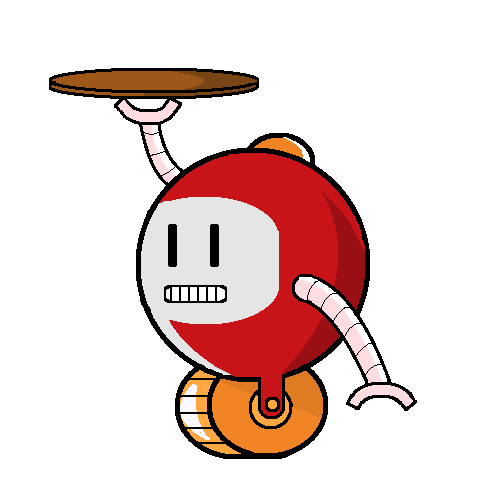
\includegraphics [scale = .3, trim={.4cm 0 .8cm 0},clip] {figures/alfred.png}
\end {figure}

{
\Huge{LazyBots} }

\vspace{1 cm}
{\Large\textbf{\textsc{McMaster University}}\\}  \vspace {1cm}
{\Large Draft Verification and Validation\\ \vspace {0.4 cm} SE 4GA6 \& TRON 4TB6}  \vspace {1cm}

{\large \textsc{Group 9} \\} \vspace{1cm}

\begin{tabular}{ l c  l}
Karim Guirguis & & 001307668 \\
David Hemms & & 001309228 \\
Marko Laban & & 001300989 \\
Curtis Milo & & 001305877 \\
Keyur Patel & & 001311559 \\
Alexandra Rahman & & 001305735
\end{tabular}




\end{center}

% --------- TITLE PAGE END------- %

\pagebreak

% Inserting table of contents and table of figures 

\tableofcontents
\listoftables
\listoffigures



\pagebreak

% -----------  REVISION HISTORY START ----------- %

%\section*{Revisions}
%\thispagestyle{empty}
\section{Revisions}
\begin{longtable}{| p{.2\textwidth } | p{.23\textwidth } | p{.23\textwidth } | p{.23\textwidth } |} \caption{LazyBots Table of Revisions}  \\

\hline 
\centering \textbf{Date} & 
\multicolumn{1}{c|}{\textbf {Revision Number}} &
\multicolumn{1}{c|}{\textbf {Authors}} & 
\multicolumn{1}{c|}{\textbf {Comments}} \\ \hline


\multicolumn{1}{|c|}{\multirow{1}{*}{\centering February 17\textsuperscript{th}, 2018}}  & 
\multirow{4}{*}{Revision 0}& 
		{Karim Guirguis \newline
		David Hemms \newline
		Marko Laban \newline
		Curtis Milo \newline
		Keyur Patel \newline
		Alexandra Rahman}
 &
 
% ------------------------------------------------------- Comments -------------------------------------------------------
\multirow{4}{*}{-} \\ 
\hline 

\end{longtable}



\pagebreak
% -------------- START INTRODUCTION ---------------- %




\section {Purpose}


The purpose of the document is to help support the development process of the drink dispensing autonomous robot known as Alfred. In particular, this document will describe what tests have been performed to ensure that Alfred will be able to perform the act of navigating to and pouring drinks correctly. 

\section {Scope}
This document will focus on different software systems that have been discussed within the system design document. This document will focus on performing tasks on the system as if it was a black box, meaning the important aspects are the inputs and outputs of the system rather then the internal mechanics. For smaller sub-features, depending on the implementation, the code may have been considered when creating test cases to ensure the system is robust. 

\section{Background}

Alfred is designed to work with various different software systems, so that it can receive the desired drinks of the user, and be able to determine based on internal knowledge of the restaurant to be able to navigate by itself to the correct table. Alfred will then have internal containment units for beverages that will allow the user to put there cup into the drink dispenser to have Alfred pour there drink for them.\\

 Alfred will be able to receive the drink that the user that the user request by requesting the next drink from a designated server. This server will story any incoming drink requests form the mobile application. This mobile application is designed to be used on a tablet or mobile device, where the servers could sign in and give it a table identification number to allow Alfred know which table has sent this order.\\
 
 Management staff will be able to view Alfred's status from the computers within the back. This system will give the management the ability to modify tables, view the errors that the robot has sent, and will allow the management staff to call Alfred back to the home base.

\section {Test Cases}

\subsection{Testing Plan and Testing Factors}
Testing was performed based on the systems and sub systems that were defined within the software. Testing was down within a bottom up approach where small unit functions were first tested. Depending on the complexity of this unit, either white box or black box testing would be chosen. If the unit was complex, white box testing would be used based to help testing based on branch coverage. Black box testing would then be used for larger integration testing. Testing was done over the following modules: \\

	\begin{longtable}{| p{0.15\textwidth} | p{0.8\textwidth} |}\hline 
				\rowcolor{tableCell}\textbf{Component} & \textbf{Test Plan Test Factors} \\ \hline
		Client Application & The main goal of testing the client application is to ensure that the experience is seamless for the customer. This means testing was done beyond just correctness testing. The bulk of the testing for the client application consisted of Usability and user interface testing. The server test cases tested the sequence in which API endpoints are accessed. Negative test cases for the client make sure that only the correct sequence of API access can be exercised.  Test numbers 01-05 focus on the pages which the staff will be interacting with (Login page and Settings page). Test number 06 tests that the customer cannot access the settings page without credentials. Test numbers 07-14 focus on testing all the components (buttons, number pickers, alerts and warnings) which the customer will be interacting with. \\ \hline
		Server & The main goal for testing the server is to make sure that all endpoints are functioning properly and return the correct results.The tests were split up into groups, based on the users of the server. Test sets within the entire test suite focused on enpoints to be used by the admin, the customers, and the robot. Another important part of testing the server was the sequence in which the endpoints were exercised. With the use of tokens and passwords, it was important to run those tests first and ensure that they went smoothly in order to proceed forward. In order for a customer to place an order, the table at which they are sitting must authenticate with the server and will be provided with a token to be used in later communication. \\ \hline
		Alfred Manager & Testing on this system was focused on unit operations working together. Test Cases were focused on Algorithms that would be used in terms of navigation. Other factors that were considered were the communication from the server to the robot as well as communication to the pumping system \\ \hline
	 	Alfred Drive-train & The main goal of testing with the drive-train system is to ensure reliability for motion in terms of navigation. Do to this, there has been a heavy amount of testing with the encoder and the open loop PWM voltage that goes to the motor, to ensure that motion is reliable and that the feedback signal is correct. From this, components were tested within a feedback loop to ensure that proper movement could be performed. Finally, the ultra sonic sensors were tested both on and off the moving robot to ensure that the system is safe if the user or something is in front of it.\\ \hline	
	 	Alfred Image Processing & The focus of the image processing system testing is within detection of circles and there proper location.  \\ \hline	
	 	Alfred Pumping System & The Alfred Pumping system focused on the mechanics of the pumps being able to receive and dispense the correct drinks, as well as detecting errors. In particular, the communication between the raspberry pi and the arduino, taking these values and dispensing the correct drink and ensuring that we are not out of liquids or that the liquids are at a non safe temperature. \\ \hline	
	\end{longtable}
\subsection{Alfred Client Application}

	\begin{longtable}{| p{0.1\textwidth} | p{0.225\textwidth} | p{0.135\textwidth} | p{0.1\textwidth} | p{.1\textwidth} | p{0.1\textwidth} | p{0.1\textwidth} |}\hline 
		\rowcolor{tableCell}\textbf{Test Number} & \textbf{Description} & \textbf{Requirement Reference} & \textbf{Inputs} & \textbf{Expected Outputs} & \textbf{Actual Outputs}& \textbf{Results} \\ \hline

01 &  Testing Login with server down &  NFR32 &  "admin:admin" as credentials &  "Could not connect to server" pop up &  "Could not connect to server" pop up &  pass
\\ \hline  
02 &  Testing Login with server running &  NFR32 &  "wrongUser: wrongPass" as credentials &  "invalid credentials" pop up &  "invalid credentials" pop up &  pass
\\ \hline  
03 &  Testing Login with server running &  NFR32 &  "admin: admin" as credentials &  settings page is launched &  settings page is launched &  pass
\\ \hline  
04 &  Testing device-table mapping change (server down) &  NFR5 &  Select different table number and click "Apply" &  "Table change unsuccessful" pop up and table number reverts to old value &  "Table change unsuccessful" pop up and table number does not revert to old value &  pass
\\ \hline  
05 &  Testing device-table mapping change (server running) &  NFR5 &  Select different table number and click "Apply" &  Drinks list page is launched &  Drinks page is launched &  pass
\\ \hline  
06 &  Testing access to settings page after initial setup &  NFR32 &  Press back after drinks page is launched &  No observed change &  no observed change &  pass
\\ \hline  
07 &  Testing drink amount selection &  NFR35\newline NFR21\newline NFR8\newline NFR5 &  Change the amount of sprite from 0 to 2 &  the number picker value will display 2 &  the number picker value displays 2 &  pass
\\ \hline  
08 &  Testing cart info &  NFR5\newline NFR21\newline NFR30\newline NFR32 &  On the drinks list page select 1 Sprite and 2 cokes and click on "Go to cart" &  current cart page is launched and the summary of items shows 1 sprite and 2 cokes &  current cart page is launched and the summary of items shows 1 sprite and 2 cokes &  pass\\ \hline  
09 &  Testing sending order to server (server down , empty cart) &  T01\newline T02\newline NFR15 &  have 0 drinks selected and click "send order" on the cart page &  "Empty cart!" pop up &  "Empty cart!" pop up &  pass
\\ \hline  
10 &  Testing sending order to server (server down , non-empty cart) &  T01\newline T02\newline NFR15 &  have some drinks selected and click "send order" on the cart page &  "Order placement unsuccessful" pop up &  "Order placement unsuccessful" pop up &  pass
\\ \hline  
11 &  Testing sending order to server (server running , empty cart) &  T01\newline T02\newline NFR15 &  0 drinks selected and click "send order" on the cart page &  "Empty cart!" pop up &  "Empty cart!" pop up &  pass
\\ \hline  
12 &  Testing sending order to server (server running , non-empty cart) &  T01\newline T02\newline NFR15 &  have some drinks selected and click "send order" on the cart page &  "Order has been received by Alfred" pop up and place in line is displayed &  "Order has been received by Alfred" pop up and place in line is displayed &  pass
\\ \hline  
13 &  Testing cart reset after order placed(drink selection page) &  N/A &  send successful order and press "back" to go to drinks page &  all drink amounts reset to 0 &  all drink amounts reset to 0 &  pass
\\ \hline  
14 &  Testing cart reset after order placed(cart page) &  N/A &  send successful order and press "back" to go to drinks page and press "go to cart" &  cart is empty &  cart is empty &  pass \\ \hline  
\end{longtable}

\subsection{Server System}

\begin{longtable}{| p{0.1\textwidth} | p{0.225\textwidth} | p{0.135\textwidth} | p{0.1\textwidth} | p{.1\textwidth} | p{0.1\textwidth} | p{0.1\textwidth} |}\hline 
	\rowcolor{tableCell}\textbf{Test Number} & \textbf{Description} & \textbf{Requirement Reference} & \textbf{Inputs} & \textbf{Expected Outputs} & \textbf{Actual Outputs}& \textbf{Results} \\ \hline

1 &  Test GET /drinks endpoint & N/A  &  N/A &  res.body == drinkTypes &  res.body == drinkTypes &  pass
\\ \hline  
2 &  Test GET /numOfTanks endpoint & N/A  &  N/A &  res.raw\_body == 3 &  res.raw\_body == 3 &  pass
\\ \hline  
3 &  Test POST /updateCreds endpoint &  NFR33 &  New admin username/password pair &  200 &  200 &  pass
\\ \hline  
4 &  Test POST /login endpoint &  NFR33 &  Admin username/password pair &  200 &  200 &  pass
\\ \hline  
5 &  Test POST /map endpoint &  AD1/AD2 &  Text file containing map contents &  200 &  200 &  pass
\\ \hline  
6 &  Test GET /map endpoint &  AD1/AD2 &  N/A &  File contents == Map received &  File contents == Map received &  pass
\\ \hline  
7 &  Test DELETE /drinks endpoint & N/A  &  Drink type &  Missing COKE &  Missing COKE &  pass
\\ \hline  
8 &  Test POST /drinks endpoint & N/A  &  Drink type and tank number &  COKE in body &  COKE in body &  pass
\\ \hline  
9 &  Test POST /table endpoint &  NFR33 &  Table ID &  "token" and "token\_type" in body &  "token" and "token\_type" in body &  pass
\\ \hline  
10 &  Test POST /placeOrder endpoint &  TO1/TO2 &  Table ID and order contents in JSON &  200 &  200 &  pass
\\ \hline  
11 &  Test GET /placeInLine endpoint &  AF14 &  Order ID and table ID &  res.raw\_body == 1 &  res.raw\_body == 1 &  pass
\\ \hline  
12 &  Test DELETE /cancelOrder endpoint & N/A  &  Order ID and table ID &  200 &  200 &  pass
\\ \hline  
13 &  Test POST /placeOrder endpoint &  TO1/TO2 &  Table ID and order contents in JSON &  200 &  200 &  pass
\\ \hline  
14 &  Test GET /checkToken endpoint &  NFR33 &  N/A &  Must return validity of token &  Includes validity of token &  pass
\\ \hline  
15 &  Test GET /map endpoint &  AF3 &  N/A &  File contents == Map received &  File contents == Map received &  pass
\\ \hline  
16 &  Test GET /nextOrder endpoint &  AF4 &  N/A &  Order should have all required keys &  Order has all required keys &  pass \\ \hline  
\end{longtable}

\subsection {Alfred Manager System}

\begin{longtable}{| p{0.1\textwidth} | p{0.225\textwidth} | p{0.135\textwidth} | p{0.1\textwidth} | p{.1\textwidth} | p{0.1\textwidth} | p{0.1\textwidth} |}\hline 
	\rowcolor{tableCell}\textbf{Test Number} & \textbf{Description} & \textbf{Requirement Reference} & \textbf{Inputs} & \textbf{Expected Outputs} & \textbf{Actual Outputs}& \textbf{Results} \\ \hline
	1 &  Testing the ability to avoid obstacles and reach 2 tables 2x4 matrix 2 obstacles &  AF3, AF10 &  map1.txt &  [[(0, 1)], [(0, 2), (1, 2)]] &  [[(0, 1)], [(0, 2), (1, 2)]] &  pass
	\\ \hline  
	2 &  Testing 3 routes to a table and 1 route to another table 3x3 matrix 1 obstacle 2 tables &  AF3, AF10 &  map2.txt & [[(1, 0), (2, 0), (2, 1), (2, 2), (1, 2)] &  [(1, 2)]], [[(1, 0), (2, 0), (2, 1), (2, 2), (1, 2)], [(1, 2)]] &  pass
	\\ \hline  
	3 &  Testing multiple routes to same table with no other tables. 3x3 matrix with 1 obstacle and 1 table &  AF3, AF10 &  map3.txt & [[(0, 1), (0, 2)]] &  [[(0, 1), (0, 2)]] &  pass
	\\ \hline  
	4 &  Testing the order of reaching tables Tables traversed by row priority and column relative to home 4x5 matrix with 3 tables and 8 obstacles &  AF3, AF10 &  map4.txt & [[(0, 1), (0, 2), (0, 3)], [(0, 2), (1, 2), (2, 2)], [(3, 2), (3, 1)]] &  [[(0, 1), (0, 2), (0, 3)], [(0, 2), (1, 2), (2, 2)], [(3, 2), (3, 1)]] &  pass
	\\ \hline  
	5 &  Testing whether an exception is thrown if table is unreachable. 2x3 matrix with 1 unreachable table, 2 obstacles &  AF3, AF10 &  map5.txt &  KeyError(" could not reach table") &  pass
	\\ \hline  
	6 &  Testing complex flow and tables in corners. 4x6 matrix with 3 tables and 7 obstacles &  AF3, AF10 &  map6.txt & [[(1, 0), (2, 0), (2, 1), (2, 2), (1, 2), (1, 3), (0, 3), (0, 4)], [(0, 3), (1, 3), (1, 2)], [(2, 2), (3, 2), (3, 3), (3, 4), (2, 4)]] &  [[(1, 0), (2, 0), (2, 1), (2, 2), (1, 2), (1, 3), (0, 3), (0, 4)], [(0, 3), (1, 3), (1, 2)], [(2, 2), (3, 2), (3, 3), (3, 4), (2, 4)]] &  pass
	\\ \hline  
	7 &  Testing complex flow, tables in corners, multiple obstacles and tables 1 spot away from each other. 5x10 matrix with 6 tables and 18 obstacles &  AF3, AF10 &  map7.txt &  [[(1, 0), (2, 0), (3, 0), (4, 0), (4, 1), (4, 2), (3, 2), (3, 3), (3, 4), (3, 5), (3, 6), (3, 7), (2, 7), (1, 7), (0, 7)], [(0, 8), (0, 9)], [(1, 9)], [], [(0, 9), (0, 8), (0, 7), (1, 7), (1, 6)], [(1, 7), (2, 7), (3, 7), (3, 6), (3, 5), (3, 4), (3, 3), (3, 2), (4, 2), (4, 1), (4, 0), (3, 0), (2, 0)]] &  [[(0, 1), (1, 1), (2, 1), (2, 0), (3, 0), (4, 0), (4, 1), (4, 2), (3, 2), (3, 3), (3, 4), (3, 5), (2, 5), (1, 5), (1, 6)], [(0, 6), (0, 7), (0, 8), (0, 9)], [(0, 8), (0, 7), (0, 6), (1, 6)], [(0, 6), (0, 7), (0, 8)], [(0, 9), (0, 10)], [(0, 9), (0, 8), (0, 7), (0, 6), (1, 6), (1, 5), (2, 5), (3, 5), (3, 4), (3, 3), (3, 2), (4, 2), (4, 1), (4, 0), (3, 0), (2, 0)]] &  fail \\ \hline  
	8 &  receiving an order &  A1 &  An order of Coke and Diet Coke on the User Application &  Alfred receives a drink that corresponds to tank 1 and 2 &  Alfred receives a drink that corresponds to tank 1 and tank 2 & Pass \\ \hline
\end{longtable}

\subsection {Alfred Drive Train System}

	\begin{longtable}{| p{0.1\textwidth} | p{0.225\textwidth} | p{0.135\textwidth} | p{0.1\textwidth} | p{.1\textwidth} | p{0.1\textwidth} | p{0.1\textwidth} |}\hline 
		\rowcolor{tableCell}\textbf{Test Number} & \textbf{Description} & \textbf{Requirement Reference} & \textbf{Inputs} & \textbf{Expected Outputs} & \textbf{Actual Outputs}& \textbf{Results} \\ \hline

		1 &  Testing Positive Change of Left Encoder & AF3 & movement of encoder &  60= 60+1 &  61 &   pass \\ \hline
		2 &  Testing Negative Change of Left Encoder & AF3 & movement of encoder &  60= 60-1 &  59 &   pass
		\\ \hline
		3 &  Testing Positive Change of Encoder &  AF3 &  movement of encoder &  60= 60+1 &  61 &   pass
		\\  \hline
		4 &  Testing Negative Change of Encoder &  AF3 &  movment of encoder &  60= 60-1 &  59 &   pass
		\\ \hline 
		5 &  Open Loop Test of Movement going forward &  AF3 &  10\% duty cycles &  Both wheels spin forward &  Both wheels spin forward &   pass
		\\ \hline
		6 &  Open Loop Test of Movement for turning &  AF3 & 10\% duty cycles with one pin on to specify backward motion &  Wheels spining in different directions &  Wheels spining in different directions &   pass
		\\ \hline
		7 &  Ultra Sonic distance test at 1.5m &  AF10 &  a wall 1.5m in front of robot &  Nothing blocking &  Nothing blocking &   pass
		\\ \hline
		8 &  Ultra Sonic distance test at 0.35m &  AF10 & a book blocking the path &  Blocked &  Blocked &   pass
		\\ \hline
	
		9 &  Speed is slewed on start &  AF3 &  A 30\% in duty cycles &  Printing showing a duty cycle increase &  Printing showing a duty cycle increase to 30\% &  pass\\ \hline
		10 &  Closed Loop Test of Movement going forward &  AF3 &  reference of 20 encoder counts/sec &  Both wheels spin forward at 20 encoder counts/s &  Both wheels spin forward at  20 encoder counts/s &   pass\\ \hline
		11 &  Closed Loop Test of Movement going forward &  AF3 &  reference of 10 encoder counts/sec &  Both wheels spin forward at  10 encoder counts/s &  Left side failed to correctly start &  fail - the software worked correctly but there was mechanical issues at slow speeds \\ \hline
		12 &  Closed Loop Test of Movement going forward with unequal resistance &  AF3 &  reference of 20 encoder counts/sec &  Both wheels spin forward at 20 encoder counts/s & Both wheels spin forward at  20 encoder counts/s &   pass
		\\ \hline
		13 &  Closed Loop Test of Movement for turning &  AF3 &  reference of 20 encoder counts/sec &  Wheels spinning in different directions at 20 encoder counts/s & Wheels spinning in different directions at 20 encoder counts/s &  pass 
		\\ \hline
		14 &  Ultra Sonic Stop &  AF3 &  reference of 20 encoder counts/sec then something blocks its path &  Something is blocking the path while moving so Alfred stops &  Alfred Stopped &  pass 
		\\ \hline

		15 &  Turn of 90deg &  AF3 &  A reference of 90 degrees &  Alfred will turn 90deg and stop &  Alfred continued to turn &  fail- needs to be re-designed.
		\\ \hline
	\end{longtable}


\subsection {Alfred Image Processing System}
\begin{longtable}{| p{0.1\textwidth} | p{0.225\textwidth} | p{0.135\textwidth} | p{0.1\textwidth} | p{.1\textwidth} | p{0.1\textwidth} | p{0.1\textwidth} |}\hline 
\rowcolor{tableCell}\textbf{Test Number} & \textbf{Description} & \textbf{Requirement Reference} & \textbf{Inputs} & \textbf{Expected Outputs} & \textbf{Actual Outputs}& \textbf{Results} \\ \hline

	9 &  Able to take picture &  AF3 & software trigger to take the picture &  A picture &  a Picture &  pass
\\ \hline
10 &  Able to detect circles from an image &  AF3 &  Image with a circle &  Position of the circle &  Position of the circle &  pass
\\ \hline
	17 &  Image processing stop with node close &  AF3 &  an image close up to camera while moving &  Has reached the next node so Alfred stops motion &  Alfred Stopped &  pass 
	\\ \hline
	18 &  Image processing stop with node at ceiling away &  AF3 &  An image further away at ceiling height distance &  Has reached the next node so Alfred stops motion &  Alfred Stopped &  Conditional pass- needed lighting
	\\ \hline
	
	\end{longtable}






\subsection {Alfred Pumping System}

	\begin{longtable}{| p{0.1\textwidth} | p{0.225\textwidth} | p{0.135\textwidth} | p{0.1\textwidth} | p{.1\textwidth} | p{0.1\textwidth} | p{0.1\textwidth} |}\hline 
		\rowcolor{tableCell}\textbf{Test Number} & \textbf{Description} & \textbf{Requirement Reference} & \textbf{Inputs} & \textbf{Expected Outputs} & \textbf{Actual Outputs}& \textbf{Results} \\ \hline
		1 &  Testing Serial communication to Arduino by sending d1d2x sent from Computer &  AF1 &  d1d2x via serial signal &  reading d1d2x read by USB & reading d1d2x read by USB &  pass
		\\ \hline  
		2 &  Testing Serial communication from RPI by sending d1d2x sent from RPI &  AF1 & d1d2x via serial signal &  reading d1d2x read by USB & reading d1d2x read by USB &  pass
		\\ \hline  
		3 &  Testing Serial communication from RPI by receiving 11110000x sent from Arduino & AF1& 11110000x via serial signal & reading 11110000x read by RPI USB & reading 11110000x read by RPI USB &  pass
		\\ \hline  
		4 &  Testing receiving a value of 20C water with the temperature sensor &  AF1 & Temperature sensor in 20C water &  20 &  19.8 &  pass
		\\ \hline  
		5 &  Testing receiving a value of 1Kg with the load sensor &  AF1 &  1kg on load cell  & 1kg &  0kg &  Fail \\ \hline  
		6 &  Able to receive from the correct tank based on drink order (Tank 1) &  AF2 &  Order for tank 1 &  Tank  1 pours &  Tank 1 pours &  pass
		\\ \hline  
		7 &  Able to receive from the correct tank based on drink order (Tank 2) &  AF2 &  Order for tank 2 &  Tank  2 pours &  Tank 2 pours &  pass
		\\ \hline  
		8 &  Able to receive from the correct tank based on drink order (Tank 3) &  AF2 &  Order for tank 3 &  Tank  3 pours &  Tank 3 pours &  pass
		\\ \hline  
		9 &  Under Weight error when tank is empty &  AF2 &  No weight &  Under Weight Error &  Nothing  &  Fail need amplifier for weight sensor
		\\ \hline  
		10 &  Over Temperature error when tank is empty &  AF2 &  a hot liquid &  Over Temperature Error &  Over Temperature Error &  Pass
		\\ \hline  
		11 &  Not over Tempature error when tank is empty &  AF2 &  a cold liquid &  No Over Temperature Error &  Nothing &  Pass \\ \hline  
	\end{longtable}



\section {Beyond Testing}

\subsection {Code Walk-through and Code Reviews}
Code reviews were performed with at least two of the software team that had not wrote the code in particular. When a new piece of code would be pushed. A review request would be made and the person who wrote the code would help explain the functionality of the software to the other group members. From there, group members would be advised to ask questions about the software and would suggest changes if needed.

\subsection {Static Analysis}
Will be performed within future revisions.

\subsection {Formal Proofs}
Will be performed on the Motor control/Image processing within future revisions.

\section {Supporting Material}

Please refer to previous design documents.

\pagebreak

\section {Appendix}
The following is the Traceability Matrix for the functional requirements: \\

\begin{longtable}{ | p{0.125\textwidth} | c | c | c | c | c | c | c | c | c | c | c | c | }
\hline
	Requirements ID: & AF1 & AF2 & AF3 & AF4 & AF5 & AF6 & AF7 & AF8 & AF9 & AF10 & AF11 & AF12 \\ \hline
	CA01 & 0 & 0 & 0 & 0 & 0 & 0 & 0 & 0 & 0 & 0 & 0 & 0 \\ \hline
	CA02 & 0 & 0 & 0 & 0 & 0 & 0 & 0 & 0 & 0 & 0 & 0 & 0 \\ \hline
	CA03 & 0 & 0 & 0 & 0 & 0 & 0 & 0 & 0 & 0 & 0 & 0 & 0 \\ \hline
	CA04 & 0 & 0 & 0 & 0 & 0 & 0 & 0 & 0 & 0 & 0 & 0 & 0 \\ \hline
	CA05 & 0 & 0 & 0 & 0 & 0 & 0 & 0 & 0 & 0 & 0 & 0 & 0 \\ \hline
	CA06 & 0 & 0 & 0 & 0 & 0 & 0 & 0 & 0 & 0 & 0 & 0 & 0 \\ \hline
	CA07 & 0 & 0 & 0 & 0 & 0 & 0 & 0 & 0 & 0 & 0 & 0 & 0 \\ \hline
	CA08 & 0 & 0 & 0 & 0 & 0 & 0 & 0 & 0 & 0 & 0 & 0 & 0 \\ \hline
	CA09 & 0 & 0 & 0 & 0 & 0 & 0 & 0 & 0 & 0 & 0 & 0 & 0 \\ \hline
	CA10 & 0 & 0 & 0 & 0 & 0 & 0 & 0 & 0 & 0 & 0 & 0 & 0 \\ \hline
	CA11 & 0 & 0 & 0 & 0 & 0 & 0 & 0 & 0 & 0 & 0 & 0 & 0 \\ \hline
	CA12 & 0 & 0 & 0 & 0 & 0 & 0 & 0 & 0 & 0 & 0 & 0 & 0 \\ \hline
	CA13 & 0 & 0 & 0 & 0 & 0 & 0 & 0 & 0 & 0 & 0 & 0 & 0 \\ \hline
	CA14 & 0 & 0 & 0 & 0 & 0 & 0 & 0 & 0 & 0 & 0 & 0 & 0 \\ \hline
	SS01 & 0 & 0 & 0 & 0 & 0 & 0 & 0 & 0 & 0 & 0 & 0 & 0 \\ \hline
	SS02 & 0 & 0 & 0 & 0 & 0 & 0 & 0 & 0 & 0 & 0 & 0 & 0 \\ \hline
	SS03 & 0 & 0 & 0 & 0 & 0 & 0 & 0 & 0 & 0 & 0 & 0 & 0 \\ \hline
	SS04 & 0 & 0 & 0 & 0 & 0 & 0 & 0 & 0 & 0 & 0 & 0 & 0 \\ \hline
	SS05 & 0 & 0 & 0 & 0 & 0 & 0 & 0 & 0 & 0 & 0 & 0 & 0 \\ \hline
	SS06 & 0 & 0 & 0 & 0 & 0 & 0 & 0 & 0 & 0 & 0 & 0 & 0 \\ \hline
	SS07 & 0 & 0 & 0 & 0 & 0 & 0 & 0 & 0 & 0 & 0 & 0 & 0 \\ \hline
	SS08 & 0 & 0 & 0 & 0 & 0 & 0 & 0 & 0 & 0 & 0 & 0 & 0 \\ \hline
	SS09 & 0 & 0 & 0 & 0 & 0 & 0 & 0 & 0 & 0 & 0 & 0 & 0 \\ \hline
	SS10 & 0 & 0 & 0 & 0 & 0 & 0 & 0 & 0 & 0 & 0 & 0 & 0 \\ \hline
	SS11 & 0 & 0 & 0 & 0 & 0 & 0 & 0 & 0 & 0 & 0 & 0 & 0 \\ \hline
	SS12 & 0 & 0 & 0 & 0 & 0 & 0 & 0 & 0 & 0 & 0 & 0 & 0 \\ \hline
	SS13 & 0 & 0 & 0 & 0 & 0 & 0 & 0 & 0 & 0 & 0 & 0 & 0 \\ \hline
	SS14 & 0 & 0 & 1 & 0 & 0 & 0 & 0 & 0 & 0 & 0 & 0 & 0 \\ \hline
	SS15 & 0 & 0 & 0 & 1 & 0 & 0 & 0 & 0 & 0 & 0 & 0 & 0 \\ \hline
	SS16 & 0 & 0 & 0 & 0 & 0 & 0 & 0 & 0 & 0 & 0 & 0 & 0 \\ \hline
	MS01 & 0 & 0 & 1 & 0 & 0 & 0 & 0 & 0 & 0 & 1 & 0 & 0 \\ \hline
	MS02 & 0 & 0 & 1 & 0 & 0 & 0 & 0 & 0 & 0 & 1 & 0 & 0 \\ \hline
	MS03 & 0 & 0 & 1 & 0 & 0 & 0 & 0 & 0 & 0 & 1 & 0 & 0 \\ \hline
	MS04 & 0 & 0 & 1 & 0 & 0 & 0 & 0 & 0 & 0 & 1 & 0 & 0 \\ \hline
	MS05 & 0 & 0 & 1 & 0 & 0 & 0 & 0 & 0 & 0 & 1 & 0 & 0 \\ \hline
	MS06 & 0 & 0 & 1 & 0 & 0 & 0 & 0 & 0 & 0 & 1 & 0 & 0 \\ \hline
	MS07 & 0 & 0 & 1 & 0 & 0 & 0 & 0 & 0 & 0 & 1 & 0 & 0 \\ \hline
	MS08 & 1 & 0 & 0 & 0 & 0 & 0 & 0 & 0 & 0 & 0 & 0 & 0 \\ \hline
	DT01 & 0 & 0 & 1 & 0 & 0 & 0 & 0 & 0 & 0 & 0 & 0 & 0 \\ \hline
	DT02 & 0 & 0 & 1 & 0 & 0 & 0 & 0 & 0 & 0 & 0 & 0 & 0 \\ \hline
	DT03 & 0 & 0 & 1 & 0 & 0 & 0 & 0 & 0 & 0 & 0 & 0 & 0 \\ \hline
	DT04 & 0 & 0 & 1 & 0 & 0 & 0 & 0 & 0 & 0 & 0 & 0 & 0 \\ \hline
	DT05 & 0 & 0 & 1 & 0 & 0 & 0 & 0 & 0 & 0 & 0 & 0 & 0 \\ \hline
	DT06 & 0 & 0 & 1 & 0 & 0 & 0 & 0 & 0 & 0 & 0 & 0 & 0 \\ \hline
	DT07 & 0 & 0 & 0 & 0 & 0 & 0 & 0 & 0 & 0 & 1 & 0 & 0 \\ \hline
	DT08 & 0 & 0 & 0 & 0 & 0 & 0 & 0 & 0 & 0 & 1 & 0 & 0 \\ \hline
	DT09 & 0 & 0 & 1 & 0 & 0 & 0 & 0 & 0 & 0 & 0 & 0 & 0 \\ \hline
	DT10 & 0 & 0 & 1 & 0 & 0 & 0 & 0 & 0 & 0 & 0 & 0 & 0 \\ \hline
	DT11 & 0 & 0 & 1 & 0 & 0 & 0 & 0 & 0 & 0 & 0 & 0 & 0 \\ \hline
	DT12 & 0 & 0 & 1 & 0 & 0 & 0 & 0 & 0 & 0 & 0 & 0 & 0 \\ \hline
	DT13 & 0 & 0 & 1 & 0 & 0 & 0 & 0 & 0 & 0 & 0 & 0 & 0 \\ \hline
	DT14 & 0 & 0 & 1 & 0 & 0 & 0 & 0 & 0 & 0 & 0 & 0 & 0 \\ \hline
	DT15 & 0 & 0 & 1 & 0 & 0 & 0 & 0 & 0 & 0 & 0 & 0 & 0 \\ \hline
	IP01 & 0 & 0 & 1 & 0 & 0 & 0 & 0 & 0 & 0 & 0 & 0 & 0 \\ \hline
	IP02 & 0 & 0 & 1 & 0 & 0 & 0 & 0 & 0 & 0 & 0 & 0 & 0 \\ \hline
	IP03 & 0 & 0 & 1 & 0 & 0 & 0 & 0 & 0 & 0 & 0 & 0 & 0 \\ \hline
	IP04 & 0 & 0 & 1 & 0 & 0 & 0 & 0 & 0 & 0 & 0 & 0 & 0 \\ \hline
	PS01 & 1 & 0 & 0 & 0 & 0 & 0 & 0 & 0 & 0 & 0 & 0 & 0 \\ \hline
	PS02 & 1 & 0 & 0 & 0 & 0 & 0 & 0 & 0 & 0 & 0 & 0 & 0 \\ \hline
	PS03 & 1 & 0 & 0 & 0 & 0 & 0 & 0 & 0 & 0 & 0 & 0 & 0 \\ \hline
	PS04 & 1 & 0 & 0 & 0 & 0 & 0 & 0 & 0 & 0 & 0 & 0 & 0 \\ \hline
	PS05 & 1 & 0 & 0 & 0 & 0 & 0 & 0 & 0 & 0 & 0 & 0 & 0 \\ \hline
	PS06 & 1 & 0 & 0 & 0 & 0 & 0 & 0 & 0 & 0 & 0 & 0 & 0 \\ \hline
	PS07 & 1 & 0 & 0 & 0 & 0 & 0 & 0 & 0 & 0 & 0 & 0 & 0 \\ \hline
	PS08 & 1 & 0 & 0 & 0 & 0 & 0 & 0 & 0 & 0 & 0 & 0 & 0 \\ \hline
	PS09 & 1 & 0 & 0 & 0 & 0 & 0 & 0 & 0 & 0 & 0 & 0 & 0 \\ \hline
	PS10 & 1 & 0 & 0 & 0 & 0 & 0 & 0 & 0 & 0 & 0 & 0 & 0 \\ \hline
	PS11 & 1 & 0 & 0 & 0 & 0 & 0 & 0 & 0 & 0 & 0 & 0 & 0 \\ \hline
\end{longtable}

\begin{longtable}{ | p{0.125\textwidth} | c | c | c | c | c | c | c | c | c | }
\hline
	Requirements ID: & AF12 & AF13 & AF14 & TO1 & TO2 & AD1 & AD2 & AD3 & AD4 \\ \hline
	CA01 & 0 & 0 & 0 & 0 & 0 & 0 & 0 & 0 & 0 \\ \hline
	CA02 & 0 & 0 & 0 & 0 & 0 & 0 & 0 & 0 & 0 \\ \hline
	CA03 & 0 & 0 & 0 & 0 & 0 & 0 & 0 & 0 & 0 \\ \hline
	CA04 & 0 & 0 & 0 & 0 & 0 & 0 & 0 & 0 & 0 \\ \hline
	CA05 & 0 & 0 & 0 & 0 & 0 & 0 & 0 & 0 & 0 \\ \hline
	CA06 & 0 & 0 & 0 & 0 & 0 & 0 & 0 & 0 & 0 \\ \hline
	CA07 & 0 & 0 & 0 & 0 & 0 & 0 & 0 & 0 & 0 \\ \hline
	CA08 & 0 & 0 & 0 & 0 & 0 & 0 & 0 & 0 & 0 \\ \hline
	CA09 & 0 & 0 & 0 & 1 & 1 & 0 & 0 & 0 & 0 \\ \hline
	CA10 & 0 & 0 & 0 & 1 & 1 & 0 & 0 & 0 & 0 \\ \hline
	CA11 & 0 & 0 & 0 & 1 & 1 & 0 & 0 & 0 & 0 \\ \hline
	CA12 & 0 & 0 & 0 & 1 & 1 & 0 & 0 & 0 & 0 \\ \hline
	CA13 & 0 & 0 & 0 & 0 & 0 & 0 & 0 & 0 & 0 \\ \hline
	CA14 & 0 & 0 & 0 & 0 & 0 & 0 & 0 & 0 & 0 \\ \hline
	SS01 & 0 & 0 & 0 & 0 & 0 & 0 & 0 & 0 & 0 \\ \hline
	SS02 & 0 & 0 & 0 & 0 & 0 & 0 & 0 & 0 & 0 \\ \hline
	SS03 & 0 & 0 & 0 & 0 & 0 & 0 & 0 & 0 & 0 \\ \hline
	SS04 & 0 & 0 & 0 & 0 & 0 & 0 & 0 & 0 & 0 \\ \hline
	SS05 & 0 & 0 & 0 & 0 & 0 & 1 & 0 & 0 & 0 \\ \hline
	SS06 & 0 & 0 & 0 & 0 & 0 & 1 & 0 & 0 & 0 \\ \hline
	SS07 & 0 & 0 & 0 & 0 & 0 & 0 & 0 & 0 & 0 \\ \hline
	SS08 & 0 & 0 & 0 & 0 & 0 & 0 & 0 & 0 & 0 \\ \hline
	SS09 & 0 & 0 & 0 & 0 & 0 & 0 & 0 & 0 & 0 \\ \hline
	SS10 & 0 & 0 & 0 & 1 & 1 & 0 & 0 & 0 & 0 \\ \hline
	SS11 & 0 & 0 & 1 & 0 & 0 & 0 & 0 & 0 & 0 \\ \hline
	SS12 & 0 & 0 & 0 & 0 & 0 & 0 & 0 & 0 & 0 \\ \hline
	SS13 & 0 & 0 & 0 & 1 & 1 & 0 & 0 & 0 & 0 \\ \hline
	SS14 & 0 & 0 & 0 & 0 & 0 & 0 & 0 & 0 & 0 \\ \hline
	SS15 & 0 & 0 & 0 & 0 & 0 & 0 & 0 & 0 & 0 \\ \hline
	SS16 & 0 & 0 & 0 & 0 & 0 & 0 & 0 & 0 & 0 \\ \hline
	MS01 & 0 & 0 & 0 & 0 & 0 & 0 & 0 & 0 & 0 \\ \hline
	MS02 & 0 & 0 & 0 & 0 & 0 & 0 & 0 & 0 & 0 \\ \hline
	MS03 & 0 & 0 & 0 & 0 & 0 & 0 & 0 & 0 & 0 \\ \hline
	MS04 & 0 & 0 & 0 & 0 & 0 & 0 & 0 & 0 & 0 \\ \hline
	MS05 & 0 & 0 & 0 & 0 & 0 & 0 & 0 & 0 & 0 \\ \hline
	MS06 & 0 & 0 & 0 & 0 & 0 & 0 & 0 & 0 & 0 \\ \hline
	MS07 & 0 & 0 & 0 & 0 & 0 & 0 & 0 & 0 & 0 \\ \hline
	MS08 & 0 & 0 & 0 & 0 & 0 & 0 & 0 & 0 & 0 \\ \hline
	DT01 & 0 & 0 & 0 & 0 & 0 & 0 & 0 & 0 & 0 \\ \hline
	DT02 & 0 & 0 & 0 & 0 & 0 & 0 & 0 & 0 & 0 \\ \hline
	DT03 & 0 & 0 & 0 & 0 & 0 & 0 & 0 & 0 & 0 \\ \hline
	DT04 & 0 & 0 & 0 & 0 & 0 & 0 & 0 & 0 & 0 \\ \hline
	DT05 & 0 & 0 & 0 & 0 & 0 & 0 & 0 & 0 & 0 \\ \hline
	DT06 & 0 & 0 & 0 & 0 & 0 & 0 & 0 & 0 & 0 \\ \hline
	DT07 & 0 & 0 & 0 & 0 & 0 & 0 & 0 & 0 & 0 \\ \hline
	DT08 & 0 & 0 & 0 & 0 & 0 & 0 & 0 & 0 & 0 \\ \hline
	DT09 & 0 & 0 & 0 & 0 & 0 & 0 & 0 & 0 & 0 \\ \hline
	DT10 & 0 & 0 & 0 & 0 & 0 & 0 & 0 & 0 & 0 \\ \hline
	DT11 & 0 & 0 & 0 & 0 & 0 & 0 & 0 & 0 & 0 \\ \hline
	DT12 & 0 & 0 & 0 & 0 & 0 & 0 & 0 & 0 & 0 \\ \hline
	DT13 & 0 & 0 & 0 & 0 & 0 & 0 & 0 & 0 & 0 \\ \hline
	DT14 & 0 & 0 & 0 & 0 & 0 & 0 & 0 & 0 & 0 \\ \hline
	DT15 & 0 & 0 & 0 & 0 & 0 & 0 & 0 & 0 & 0 \\ \hline
	IP01 & 0 & 0 & 0 & 0 & 0 & 0 & 0 & 0 & 0 \\ \hline
	IP02 & 0 & 0 & 0 & 0 & 0 & 0 & 0 & 0 & 0 \\ \hline
	IP03 & 0 & 0 & 0 & 0 & 0 & 0 & 0 & 0 & 0 \\ \hline
	IP04 & 0 & 0 & 0 & 0 & 0 & 0 & 0 & 0 & 0 \\ \hline
	PS01 & 0 & 0 & 0 & 0 & 0 & 0 & 0 & 0 & 0 \\ \hline
	PS02 & 0 & 0 & 0 & 0 & 0 & 0 & 0 & 0 & 0 \\ \hline
	PS03 & 0 & 0 & 0 & 0 & 0 & 0 & 0 & 0 & 0 \\ \hline
	PS04 & 0 & 0 & 0 & 0 & 0 & 0 & 0 & 0 & 0 \\ \hline
	PS05 & 0 & 0 & 0 & 0 & 0 & 0 & 0 & 0 & 0 \\ \hline
	PS06 & 0 & 0 & 0 & 0 & 0 & 0 & 0 & 0 & 0 \\ \hline
	PS07 & 0 & 0 & 0 & 0 & 0 & 0 & 0 & 0 & 0 \\ \hline
	PS08 & 0 & 0 & 0 & 0 & 0 & 0 & 0 & 0 & 0 \\ \hline
	PS09 & 0 & 0 & 0 & 0 & 0 & 0 & 0 & 0 & 0 \\ \hline
	PS10 & 0 & 0 & 0 & 0 & 0 & 0 & 0 & 0 & 0 \\ \hline
	PS11 & 0 & 0 & 0 & 0 & 0 & 0 & 0 & 0 & 0 \\ \hline
\end{longtable}

The following is the Traceability Matrix for the non-functional requirements: \\

\begin{longtable}{ | p{0.125\textwidth}  | c | c | c | c | c | c | c | c | c | c | c | c | }
\hline
	Requirements ID: & NFR1 & NFR2 & NFR3 & NFR4 & NFR5 & NFR6 & NFR7 & NFR8 & NFR9 & NFR10 \\ \hline
	CA01 & 0 & 0 & 0 & 0 & 0 & 0 & 0 & 0 & 0 & 0 \\ \hline
	CA02 & 0 & 0 & 0 & 0 & 0 & 0 & 0 & 0 & 0 & 0 \\ \hline
	CA03 & 0 & 0 & 0 & 0 & 0 & 0 & 0 & 0 & 0 & 0 \\ \hline
	CA04 & 0 & 0 & 0 & 0 & 1 & 0 & 0 & 0 & 0 & 0 \\ \hline
	CA05 & 0 & 0 & 0 & 0 & 1 & 0 & 0 & 0 & 0 & 0 \\ \hline
	CA06 & 0 & 0 & 0 & 0 & 0 & 0 & 0 & 0 & 0 & 0 \\ \hline
	CA07 & 0 & 0 & 0 & 0 & 1 & 0 & 0 & 1 & 0 & 0 \\ \hline
	CA08 & 0 & 0 & 0 & 0 & 1 & 0 & 0 & 0 & 0 & 0 \\ \hline
	CA09 & 0 & 0 & 0 & 0 & 0 & 0 & 0 & 0 & 0 & 0 \\ \hline
	CA10 & 0 & 0 & 0 & 0 & 0 & 0 & 0 & 0 & 0 & 0 \\ \hline
	CA11 & 0 & 0 & 0 & 0 & 0 & 0 & 0 & 0 & 0 & 0 \\ \hline
	CA12 & 0 & 0 & 0 & 0 & 0 & 0 & 0 & 0 & 0 & 0 \\ \hline
	CA13 & 0 & 0 & 0 & 0 & 0 & 0 & 0 & 0 & 0 & 0 \\ \hline
	CA14 & 0 & 0 & 0 & 0 & 0 & 0 & 0 & 0 & 0 & 0 \\ \hline
	SS01 & 0 & 0 & 0 & 0 & 0 & 0 & 0 & 0 & 0 & 0 \\ \hline
	SS02 & 0 & 0 & 0 & 0 & 0 & 0 & 0 & 0 & 0 & 0 \\ \hline
	SS03 & 0 & 0 & 0 & 0 & 0 & 0 & 0 & 0 & 0 & 0 \\ \hline
	SS04 & 0 & 0 & 0 & 0 & 0 & 0 & 0 & 0 & 0 & 0 \\ \hline
	SS05 & 0 & 0 & 0 & 0 & 0 & 0 & 0 & 0 & 0 & 0 \\ \hline
	SS06 & 0 & 0 & 0 & 0 & 0 & 0 & 0 & 0 & 0 & 0 \\ \hline
	SS07 & 0 & 0 & 0 & 0 & 0 & 0 & 0 & 0 & 0 & 0 \\ \hline
	SS08 & 0 & 0 & 0 & 0 & 0 & 0 & 0 & 0 & 0 & 0 \\ \hline
	SS09 & 0 & 0 & 0 & 0 & 0 & 0 & 0 & 0 & 0 & 0 \\ \hline
	SS10 & 0 & 0 & 0 & 0 & 0 & 0 & 0 & 0 & 0 & 0 \\ \hline
	SS11 & 0 & 0 & 0 & 0 & 0 & 0 & 0 & 0 & 0 & 0 \\ \hline
	SS12 & 0 & 0 & 0 & 0 & 0 & 0 & 0 & 0 & 0 & 0 \\ \hline
	SS13 & 0 & 0 & 0 & 0 & 0 & 0 & 0 & 0 & 0 & 0 \\ \hline
	SS14 & 0 & 0 & 0 & 0 & 0 & 0 & 0 & 0 & 0 & 0 \\ \hline
	SS15 & 0 & 0 & 0 & 0 & 0 & 0 & 0 & 0 & 0 & 0 \\ \hline
	SS16 & 0 & 0 & 0 & 0 & 0 & 0 & 0 & 0 & 0 & 0 \\ \hline
	MS01 & 0 & 0 & 0 & 0 & 0 & 0 & 0 & 0 & 0 & 0 \\ \hline
	MS02 & 0 & 0 & 0 & 0 & 0 & 0 & 0 & 0 & 0 & 0 \\ \hline
	MS03 & 0 & 0 & 0 & 0 & 0 & 0 & 0 & 0 & 0 & 0 \\ \hline
	MS04 & 0 & 0 & 0 & 0 & 0 & 0 & 0 & 0 & 0 & 0 \\ \hline
	MS05 & 0 & 0 & 0 & 0 & 0 & 0 & 0 & 0 & 0 & 0 \\ \hline
	MS06 & 0 & 0 & 0 & 0 & 0 & 0 & 0 & 0 & 0 & 0 \\ \hline
	MS07 & 0 & 0 & 0 & 0 & 0 & 0 & 0 & 0 & 0 & 0 \\ \hline
	MS08 & 0 & 0 & 0 & 0 & 0 & 0 & 0 & 0 & 0 & 0 \\ \hline
	DT01 & 0 & 0 & 0 & 0 & 0 & 0 & 0 & 0 & 0 & 0 \\ \hline
	DT02 & 0 & 0 & 0 & 0 & 0 & 0 & 0 & 0 & 0 & 0 \\ \hline
	DT03 & 0 & 0 & 0 & 0 & 0 & 0 & 0 & 0 & 0 & 0 \\ \hline
	DT04 & 0 & 0 & 0 & 0 & 0 & 0 & 0 & 0 & 0 & 0 \\ \hline
	DT05 & 0 & 0 & 0 & 0 & 0 & 0 & 0 & 0 & 0 & 0 \\ \hline
	DT06 & 0 & 0 & 0 & 0 & 0 & 0 & 0 & 0 & 0 & 0 \\ \hline
	DT07 & 0 & 0 & 0 & 0 & 0 & 0 & 0 & 0 & 0 & 0 \\ \hline
	DT08 & 0 & 0 & 0 & 0 & 0 & 0 & 0 & 0 & 0 & 0 \\ \hline
	DT09 & 0 & 0 & 0 & 0 & 0 & 0 & 0 & 0 & 0 & 0 \\ \hline
	DT10 & 0 & 0 & 0 & 0 & 0 & 0 & 0 & 0 & 0 & 0 \\ \hline
	DT11 & 0 & 0 & 0 & 0 & 0 & 0 & 0 & 0 & 0 & 0 \\ \hline
	DT12 & 0 & 0 & 0 & 0 & 0 & 0 & 0 & 0 & 0 & 0 \\ \hline
	DT13 & 0 & 0 & 0 & 0 & 0 & 0 & 0 & 0 & 0 & 0 \\ \hline
	DT14 & 0 & 0 & 0 & 0 & 0 & 0 & 0 & 0 & 0 & 0 \\ \hline
	DT15 & 0 & 0 & 0 & 0 & 0 & 0 & 0 & 0 & 0 & 0 \\ \hline
	IP01 & 0 & 0 & 0 & 0 & 0 & 0 & 0 & 0 & 0 & 0 \\ \hline
	IP02 & 0 & 0 & 0 & 0 & 0 & 0 & 0 & 0 & 0 & 0 \\ \hline
	IP03 & 0 & 0 & 0 & 0 & 0 & 0 & 0 & 0 & 0 & 0 \\ \hline
	IP04 & 0 & 0 & 0 & 0 & 0 & 0 & 0 & 0 & 0 & 0 \\ \hline
	PS01 & 0 & 0 & 0 & 0 & 0 & 0 & 0 & 0 & 0 & 0 \\ \hline
	PS02 & 0 & 0 & 0 & 0 & 0 & 0 & 0 & 0 & 0 & 0 \\ \hline
	PS03 & 0 & 0 & 0 & 0 & 0 & 0 & 0 & 0 & 0 & 0 \\ \hline
	PS04 & 0 & 0 & 0 & 0 & 0 & 0 & 0 & 0 & 0 & 0 \\ \hline
	PS05 & 0 & 0 & 0 & 0 & 0 & 0 & 0 & 0 & 0 & 0 \\ \hline
	PS06 & 0 & 0 & 0 & 0 & 0 & 0 & 0 & 0 & 0 & 0 \\ \hline
	PS07 & 0 & 0 & 0 & 0 & 0 & 0 & 0 & 0 & 0 & 0 \\ \hline
\end{longtable}

\begin{longtable}{ | p{0.125\textwidth}  | c | c | c | c | c | c | c | c | c | c | }
\hline
	Requirements ID: & NFR11 & NFR12 & NFR13 & NFR14 & NFR15 & NFR16 & NFR17 & NFR18 & NFR19 & NFR20 \\ \hline
	CA01 & 0 & 0 & 0 & 0 & 0 & 0 & 0 & 0 & 0 & 0 \\ \hline
	CA02 & 0 & 0 & 0 & 0 & 0 & 0 & 0 & 0 & 0 & 0 \\ \hline
	CA03 & 0 & 0 & 0 & 0 & 0 & 0 & 0 & 0 & 0 & 0 \\ \hline
	CA04 & 0 & 0 & 0 & 0 & 0 & 0 & 0 & 0 & 0 & 0 \\ \hline
	CA05 & 0 & 0 & 0 & 0 & 0 & 0 & 0 & 0 & 0 & 0 \\ \hline
	CA06 & 0 & 0 & 0 & 0 & 0 & 0 & 0 & 0 & 0 & 0 \\ \hline
	CA07 & 0 & 0 & 0 & 0 & 0 & 0 & 0 & 0 & 0 & 0 \\ \hline
	CA08 & 0 & 0 & 0 & 0 & 0 & 0 & 0 & 0 & 0 & 0 \\ \hline
	CA09 & 0 & 0 & 0 & 0 & 1 & 0 & 0 & 0 & 0 & 0 \\ \hline
	CA10 & 0 & 0 & 0 & 0 & 1 & 0 & 0 & 0 & 0 & 0 \\ \hline
	CA11 & 0 & 0 & 0 & 0 & 1 & 0 & 0 & 0 & 0 & 0 \\ \hline
	CA12 & 0 & 0 & 0 & 0 & 1 & 0 & 0 & 0 & 0 & 0 \\ \hline
	CA13 & 0 & 0 & 0 & 0 & 0 & 0 & 0 & 0 & 0 & 0 \\ \hline
	CA14 & 0 & 0 & 0 & 0 & 0 & 0 & 0 & 0 & 0 & 0 \\ \hline
	SS01 & 0 & 0 & 0 & 0 & 0 & 0 & 0 & 0 & 0 & 0 \\ \hline
	SS02 & 0 & 0 & 0 & 0 & 0 & 0 & 0 & 0 & 0 & 0 \\ \hline
	SS03 & 0 & 0 & 0 & 0 & 0 & 0 & 0 & 0 & 0 & 0 \\ \hline
	SS04 & 0 & 0 & 0 & 0 & 0 & 0 & 0 & 0 & 0 & 0 \\ \hline
	SS05 & 0 & 0 & 0 & 0 & 0 & 0 & 0 & 0 & 0 & 0 \\ \hline
	SS06 & 0 & 0 & 0 & 0 & 0 & 0 & 0 & 0 & 0 & 0 \\ \hline
	SS07 & 0 & 0 & 0 & 0 & 0 & 0 & 0 & 0 & 0 & 0 \\ \hline
	SS08 & 0 & 0 & 0 & 0 & 0 & 0 & 0 & 0 & 0 & 0 \\ \hline
	SS09 & 0 & 0 & 0 & 0 & 0 & 0 & 0 & 0 & 0 & 0 \\ \hline
	SS10 & 0 & 0 & 0 & 0 & 0 & 0 & 0 & 0 & 0 & 0 \\ \hline
	SS11 & 0 & 0 & 0 & 0 & 0 & 0 & 0 & 0 & 0 & 0 \\ \hline
	SS12 & 0 & 0 & 0 & 0 & 0 & 0 & 0 & 0 & 0 & 0 \\ \hline
	SS13 & 0 & 0 & 0 & 0 & 0 & 0 & 0 & 0 & 0 & 0 \\ \hline
	SS14 & 0 & 0 & 0 & 0 & 0 & 0 & 0 & 0 & 0 & 0 \\ \hline
	SS15 & 0 & 0 & 0 & 0 & 0 & 0 & 0 & 0 & 0 & 0 \\ \hline
	SS16 & 0 & 0 & 0 & 0 & 0 & 0 & 0 & 0 & 0 & 0 \\ \hline
	MS01 & 0 & 0 & 0 & 0 & 0 & 0 & 0 & 0 & 0 & 0 \\ \hline
	MS02 & 0 & 0 & 0 & 0 & 0 & 0 & 0 & 0 & 0 & 0 \\ \hline
	MS03 & 0 & 0 & 0 & 0 & 0 & 0 & 0 & 0 & 0 & 0 \\ \hline
	MS04 & 0 & 0 & 0 & 0 & 0 & 0 & 0 & 0 & 0 & 0 \\ \hline
	MS05 & 0 & 0 & 0 & 0 & 0 & 0 & 0 & 0 & 0 & 0 \\ \hline
	MS06 & 0 & 0 & 0 & 0 & 0 & 0 & 0 & 0 & 0 & 0 \\ \hline
	MS07 & 0 & 0 & 0 & 0 & 0 & 0 & 0 & 0 & 0 & 0 \\ \hline
	MS08 & 0 & 0 & 0 & 0 & 0 & 0 & 0 & 0 & 0 & 0 \\ \hline
	DT01 & 0 & 0 & 0 & 0 & 0 & 0 & 0 & 0 & 0 & 0 \\ \hline
	DT02 & 0 & 0 & 0 & 0 & 0 & 0 & 0 & 0 & 0 & 0 \\ \hline
	DT03 & 0 & 0 & 0 & 0 & 0 & 0 & 0 & 0 & 0 & 0 \\ \hline
	DT04 & 0 & 0 & 0 & 0 & 0 & 0 & 0 & 0 & 0 & 0 \\ \hline
	DT05 & 0 & 0 & 0 & 0 & 0 & 0 & 0 & 0 & 0 & 0 \\ \hline
	DT06 & 0 & 0 & 0 & 0 & 0 & 0 & 0 & 0 & 0 & 0 \\ \hline
	DT07 & 0 & 0 & 0 & 0 & 0 & 0 & 0 & 0 & 0 & 0 \\ \hline
	DT08 & 0 & 0 & 0 & 0 & 0 & 0 & 0 & 0 & 0 & 0 \\ \hline
	DT09 & 0 & 0 & 0 & 0 & 0 & 0 & 0 & 0 & 0 & 0 \\ \hline
	DT10 & 0 & 0 & 0 & 0 & 0 & 0 & 0 & 0 & 0 & 0 \\ \hline
	DT11 & 0 & 0 & 0 & 0 & 0 & 0 & 0 & 0 & 0 & 0 \\ \hline
	DT12 & 0 & 0 & 0 & 0 & 0 & 0 & 0 & 0 & 0 & 0 \\ \hline
	DT13 & 0 & 0 & 0 & 0 & 0 & 0 & 0 & 0 & 0 & 0 \\ \hline
	DT14 & 0 & 0 & 0 & 0 & 0 & 0 & 0 & 0 & 0 & 0 \\ \hline
	DT15 & 0 & 0 & 0 & 0 & 0 & 0 & 0 & 0 & 0 & 0 \\ \hline
	IP01 & 0 & 0 & 0 & 0 & 0 & 0 & 0 & 0 & 0 & 0 \\ \hline
	IP02 & 0 & 0 & 0 & 0 & 0 & 0 & 0 & 0 & 0 & 0 \\ \hline
	IP03 & 0 & 0 & 0 & 0 & 0 & 0 & 0 & 0 & 0 & 0 \\ \hline
	IP04 & 0 & 0 & 0 & 0 & 0 & 0 & 0 & 0 & 0 & 0 \\ \hline
	PS01 & 0 & 0 & 0 & 0 & 0 & 0 & 0 & 0 & 0 & 0 \\ \hline
	PS02 & 0 & 0 & 0 & 0 & 0 & 0 & 0 & 0 & 0 & 0 \\ \hline
	PS03 & 0 & 0 & 0 & 0 & 0 & 0 & 0 & 0 & 0 & 0 \\ \hline
	PS04 & 0 & 0 & 0 & 0 & 0 & 0 & 0 & 0 & 0 & 0 \\ \hline
	PS05 & 0 & 0 & 0 & 0 & 0 & 0 & 0 & 0 & 0 & 0 \\ \hline
	PS06 & 0 & 0 & 0 & 0 & 0 & 0 & 0 & 0 & 0 & 0 \\ \hline
	PS07 & 0 & 0 & 0 & 0 & 0 & 0 & 0 & 0 & 0 & 0 \\ \hline
\end{longtable}

\begin{longtable}{ | p{0.125\textwidth} | c | c | c | c | c | c | c | c | c | c | }
\hline
	Requirements ID: & NFR21 & NFR22 & NFR23 & NFR24 & NFR25 & NFR26 & NFR27 & NFR28 & NFR29 & NFR30 \\ \hline
	CA01 & 0 & 0 & 0 & 0 & 0 & 0 & 0 & 0 & 0 & 0 \\ \hline
	CA02 & 0 & 0 & 0 & 0 & 0 & 0 & 0 & 0 & 0 & 0 \\ \hline
	CA03 & 0 & 0 & 0 & 0 & 0 & 0 & 0 & 0 & 0 & 0 \\ \hline
	CA04 & 0 & 0 & 0 & 0 & 0 & 0 & 0 & 0 & 0 & 0 \\ \hline
	CA05 & 0 & 0 & 0 & 0 & 0 & 0 & 0 & 0 & 0 & 0 \\ \hline
	CA06 & 0 & 0 & 0 & 0 & 0 & 0 & 0 & 0 & 0 & 0 \\ \hline
	CA07 & 1 & 0 & 0 & 0 & 0 & 0 & 0 & 0 & 0 & 0 \\ \hline
	CA08 & 1 & 0 & 0 & 0 & 0 & 0 & 0 & 0 & 0 & 1 \\ \hline
	CA09 & 0 & 0 & 0 & 0 & 0 & 0 & 0 & 0 & 0 & 0 \\ \hline
	CA10 & 0 & 0 & 0 & 0 & 0 & 0 & 0 & 0 & 0 & 0 \\ \hline
	CA11 & 0 & 0 & 0 & 0 & 0 & 0 & 0 & 0 & 0 & 0 \\ \hline
	CA12 & 0 & 0 & 0 & 0 & 0 & 0 & 0 & 0 & 0 & 0 \\ \hline
	CA13 & 0 & 0 & 0 & 0 & 0 & 0 & 0 & 0 & 0 & 0 \\ \hline
	CA14 & 0 & 0 & 0 & 0 & 0 & 0 & 0 & 0 & 0 & 0 \\ \hline
	SS01 & 0 & 0 & 0 & 0 & 0 & 0 & 0 & 0 & 0 & 0 \\ \hline
	SS02 & 0 & 0 & 0 & 0 & 0 & 0 & 0 & 0 & 0 & 0 \\ \hline
	SS03 & 0 & 0 & 0 & 0 & 0 & 0 & 0 & 0 & 0 & 0 \\ \hline
	SS04 & 0 & 0 & 0 & 0 & 0 & 0 & 0 & 0 & 0 & 0 \\ \hline
	SS05 & 0 & 0 & 0 & 0 & 0 & 0 & 0 & 0 & 0 & 0 \\ \hline
	SS06 & 0 & 0 & 0 & 0 & 0 & 0 & 0 & 0 & 0 & 0 \\ \hline
	SS07 & 0 & 0 & 0 & 0 & 0 & 0 & 0 & 0 & 0 & 0 \\ \hline
	SS08 & 0 & 0 & 0 & 0 & 0 & 0 & 0 & 0 & 0 & 0 \\ \hline
	SS09 & 0 & 0 & 0 & 0 & 0 & 0 & 0 & 0 & 0 & 0 \\ \hline
	SS10 & 0 & 0 & 0 & 0 & 0 & 0 & 0 & 0 & 0 & 0 \\ \hline
	SS11 & 0 & 0 & 0 & 0 & 0 & 0 & 0 & 0 & 0 & 0 \\ \hline
	SS12 & 0 & 0 & 0 & 0 & 0 & 0 & 0 & 0 & 0 & 0 \\ \hline
	SS13 & 0 & 0 & 0 & 0 & 0 & 0 & 0 & 0 & 0 & 0 \\ \hline
	SS14 & 0 & 0 & 0 & 0 & 0 & 0 & 0 & 0 & 0 & 0 \\ \hline
	SS15 & 0 & 0 & 0 & 0 & 0 & 0 & 0 & 0 & 0 & 0 \\ \hline
	SS16 & 0 & 0 & 0 & 0 & 0 & 0 & 0 & 0 & 0 & 0 \\ \hline
	MS01 & 0 & 0 & 0 & 0 & 0 & 0 & 0 & 0 & 0 & 0 \\ \hline
	MS02 & 0 & 0 & 0 & 0 & 0 & 0 & 0 & 0 & 0 & 0 \\ \hline
	MS03 & 0 & 0 & 0 & 0 & 0 & 0 & 0 & 0 & 0 & 0 \\ \hline
	MS04 & 0 & 0 & 0 & 0 & 0 & 0 & 0 & 0 & 0 & 0 \\ \hline
	MS05 & 0 & 0 & 0 & 0 & 0 & 0 & 0 & 0 & 0 & 0 \\ \hline
	MS06 & 0 & 0 & 0 & 0 & 0 & 0 & 0 & 0 & 0 & 0 \\ \hline
	MS07 & 0 & 0 & 0 & 0 & 0 & 0 & 0 & 0 & 0 & 0 \\ \hline
	MS08 & 0 & 0 & 0 & 0 & 0 & 0 & 0 & 0 & 0 & 0 \\ \hline
	DT01 & 0 & 0 & 0 & 0 & 0 & 0 & 0 & 0 & 0 & 0 \\ \hline
	DT02 & 0 & 0 & 0 & 0 & 0 & 0 & 0 & 0 & 0 & 0 \\ \hline
	DT03 & 0 & 0 & 0 & 0 & 0 & 0 & 0 & 0 & 0 & 0 \\ \hline
	DT04 & 0 & 0 & 0 & 0 & 0 & 0 & 0 & 0 & 0 & 0 \\ \hline
	DT05 & 0 & 0 & 0 & 0 & 0 & 0 & 0 & 0 & 0 & 0 \\ \hline
	DT06 & 0 & 0 & 0 & 0 & 0 & 0 & 0 & 0 & 0 & 0 \\ \hline
	DT07 & 0 & 0 & 0 & 0 & 0 & 0 & 0 & 0 & 0 & 0 \\ \hline
	DT08 & 0 & 0 & 0 & 0 & 0 & 0 & 0 & 0 & 0 & 0 \\ \hline
	DT09 & 0 & 0 & 0 & 0 & 0 & 0 & 0 & 0 & 0 & 0 \\ \hline
	DT10 & 0 & 0 & 0 & 0 & 0 & 0 & 0 & 0 & 0 & 0 \\ \hline
	DT11 & 0 & 0 & 0 & 0 & 0 & 0 & 0 & 0 & 0 & 0 \\ \hline
	DT12 & 0 & 0 & 0 & 0 & 0 & 0 & 0 & 0 & 0 & 0 \\ \hline
	DT13 & 0 & 0 & 0 & 0 & 0 & 0 & 0 & 0 & 0 & 0 \\ \hline
	DT14 & 0 & 0 & 0 & 0 & 0 & 0 & 0 & 0 & 0 & 0 \\ \hline
	DT15 & 0 & 0 & 0 & 0 & 0 & 0 & 0 & 0 & 0 & 0 \\ \hline
	IP01 & 0 & 0 & 0 & 0 & 0 & 0 & 0 & 0 & 0 & 0 \\ \hline
	IP02 & 0 & 0 & 0 & 0 & 0 & 0 & 0 & 0 & 0 & 0 \\ \hline
	IP03 & 0 & 0 & 0 & 0 & 0 & 0 & 0 & 0 & 0 & 0 \\ \hline
	IP04 & 0 & 0 & 0 & 0 & 0 & 0 & 0 & 0 & 0 & 0 \\ \hline
	PS01 & 0 & 0 & 0 & 0 & 0 & 0 & 0 & 0 & 0 & 0 \\ \hline
	PS02 & 0 & 0 & 0 & 0 & 0 & 0 & 0 & 0 & 0 & 0 \\ \hline
	PS03 & 0 & 0 & 0 & 0 & 0 & 0 & 0 & 0 & 0 & 0 \\ \hline
	PS04 & 0 & 0 & 0 & 0 & 0 & 0 & 0 & 0 & 0 & 0 \\ \hline
	PS05 & 0 & 0 & 0 & 0 & 0 & 0 & 0 & 0 & 0 & 0 \\ \hline
	PS06 & 0 & 0 & 0 & 0 & 0 & 0 & 0 & 0 & 0 & 0 \\ \hline
	PS07 & 0 & 0 & 0 & 0 & 0 & 0 & 0 & 0 & 0 & 0 \\ \hline
\end{longtable}

\begin{longtable}{ | p{0.125\textwidth} | c | c | c | c | c | c | c | c | }
\hline
	Requirements ID: & NFR31 & NFR32 & NFR33 & NFR34 & NFR35 & NFR36 & NFR37 & NFR38 \\ \hline
	CA01 & 0 & 1 & 0 & 0 & 0 & 0 & 0 & 0 \\ \hline
	CA02 & 0 & 1 & 0 & 0 & 0 & 0 & 0 & 0 \\ \hline
	CA03 & 0 & 1 & 0 & 0 & 0 & 0 & 0 & 0 \\ \hline
	CA04 & 0 & 0 & 0 & 0 & 0 & 0 & 0 & 0 \\ \hline
	CA05 & 0 & 0 & 0 & 0 & 0 & 0 & 0 & 0 \\ \hline
	CA06 & 0 & 1 & 0 & 0 & 0 & 0 & 0 & 0 \\ \hline
	CA07 & 0 & 0 & 0 & 0 & 1 & 0 & 0 & 0 \\ \hline
	CA08 & 0 & 1 & 0 & 0 & 0 & 0 & 0 & 0 \\ \hline
	CA09 & 0 & 0 & 0 & 0 & 0 & 0 & 0 & 0 \\ \hline
	CA10 & 0 & 0 & 0 & 0 & 0 & 0 & 0 & 0 \\ \hline
	CA11 & 0 & 0 & 0 & 0 & 0 & 0 & 0 & 0 \\ \hline
	CA12 & 0 & 0 & 0 & 0 & 0 & 0 & 0 & 0 \\ \hline
	CA13 & 0 & 0 & 0 & 0 & 0 & 0 & 0 & 0 \\ \hline
	CA14 & 0 & 0 & 0 & 0 & 0 & 0 & 0 & 0 \\ \hline
	SS01 & 0 & 0 & 0 & 0 & 0 & 0 & 0 & 0 \\ \hline
	SS02 & 0 & 0 & 0 & 0 & 0 & 0 & 0 & 0 \\ \hline
	SS03 & 0 & 0 & 1 & 0 & 0 & 0 & 0 & 0 \\ \hline
	SS04 & 0 & 0 & 1 & 0 & 0 & 0 & 0 & 0 \\ \hline
	SS05 & 0 & 0 & 0 & 0 & 0 & 0 & 0 & 0 \\ \hline
	SS06 & 0 & 0 & 0 & 0 & 0 & 0 & 0 & 0 \\ \hline
	SS07 & 0 & 0 & 0 & 0 & 0 & 0 & 0 & 0 \\ \hline
	SS08 & 0 & 0 & 0 & 0 & 0 & 0 & 0 & 0 \\ \hline
	SS09 & 0 & 0 & 1 & 0 & 0 & 0 & 0 & 0 \\ \hline
	SS10 & 0 & 0 & 0 & 0 & 0 & 0 & 0 & 0 \\ \hline
	SS11 & 0 & 0 & 0 & 0 & 0 & 0 & 0 & 0 \\ \hline
	SS12 & 0 & 0 & 0 & 0 & 0 & 0 & 0 & 0 \\ \hline
	SS13 & 0 & 0 & 0 & 0 & 0 & 0 & 0 & 0 \\ \hline
	SS14 & 0 & 0 & 1 & 0 & 0 & 0 & 0 & 0 \\ \hline
	SS15 & 0 & 0 & 0 & 0 & 0 & 0 & 0 & 0 \\ \hline
	SS16 & 0 & 0 & 0 & 0 & 0 & 0 & 0 & 0 \\ \hline
	MS01 & 0 & 0 & 0 & 0 & 0 & 0 & 0 & 0 \\ \hline
	MS02 & 0 & 0 & 0 & 0 & 0 & 0 & 0 & 0 \\ \hline
	MS03 & 0 & 0 & 0 & 0 & 0 & 0 & 0 & 0 \\ \hline
	MS04 & 0 & 0 & 0 & 0 & 0 & 0 & 0 & 0 \\ \hline
	MS05 & 0 & 0 & 0 & 0 & 0 & 0 & 0 & 0 \\ \hline
	MS06 & 0 & 0 & 0 & 0 & 0 & 0 & 0 & 0 \\ \hline
	MS07 & 0 & 0 & 0 & 0 & 0 & 0 & 0 & 0 \\ \hline
	MS08 & 0 & 0 & 0 & 0 & 0 & 0 & 0 & 0 \\ \hline
	DT01 & 0 & 0 & 0 & 0 & 0 & 0 & 0 & 0 \\ \hline
	DT02 & 0 & 0 & 0 & 0 & 0 & 0 & 0 & 0 \\ \hline
	DT03 & 0 & 0 & 0 & 0 & 0 & 0 & 0 & 0 \\ \hline
	DT04 & 0 & 0 & 0 & 0 & 0 & 0 & 0 & 0 \\ \hline
	DT05 & 0 & 0 & 0 & 0 & 0 & 0 & 0 & 0 \\ \hline
	DT06 & 0 & 0 & 0 & 0 & 0 & 0 & 0 & 0 \\ \hline
	DT07 & 0 & 0 & 0 & 0 & 0 & 0 & 0 & 0 \\ \hline
	DT08 & 0 & 0 & 0 & 0 & 0 & 0 & 0 & 0 \\ \hline
	DT09 & 0 & 0 & 0 & 0 & 0 & 0 & 0 & 0 \\ \hline
	DT10 & 0 & 0 & 0 & 0 & 0 & 0 & 0 & 0 \\ \hline
	DT11 & 0 & 0 & 0 & 0 & 0 & 0 & 0 & 0 \\ \hline
	DT12 & 0 & 0 & 0 & 0 & 0 & 0 & 0 & 0 \\ \hline
	DT13 & 0 & 0 & 0 & 0 & 0 & 0 & 0 & 0 \\ \hline
	DT14 & 0 & 0 & 0 & 0 & 0 & 0 & 0 & 0 \\ \hline
	DT15 & 0 & 0 & 0 & 0 & 0 & 0 & 0 & 0 \\ \hline
	IP01 & 0 & 0 & 0 & 0 & 0 & 0 & 0 & 0 \\ \hline
	IP02 & 0 & 0 & 0 & 0 & 0 & 0 & 0 & 0 \\ \hline
	IP03 & 0 & 0 & 0 & 0 & 0 & 0 & 0 & 0 \\ \hline
	IP04 & 0 & 0 & 0 & 0 & 0 & 0 & 0 & 0 \\ \hline
	PS01 & 0 & 0 & 0 & 0 & 0 & 0 & 0 & 0 \\ \hline
	PS02 & 0 & 0 & 0 & 0 & 0 & 0 & 0 & 0 \\ \hline
	PS03 & 0 & 0 & 0 & 0 & 0 & 0 & 0 & 0 \\ \hline
	PS04 & 0 & 0 & 0 & 0 & 0 & 0 & 0 & 0 \\ \hline
	PS05 & 0 & 0 & 0 & 0 & 0 & 0 & 0 & 0 \\ \hline
	PS06 & 0 & 0 & 0 & 0 & 0 & 0 & 0 & 0 \\ \hline
	PS07 & 0 & 0 & 0 & 0 & 0 & 0 & 0 & 0 \\ \hline
\end{longtable}


\end{document}


















